\section{Extended limitations}\label{app:limitations}
\textbf{Silent wrongs are reduced and post-hoc localized, not eliminated.} \swResidual{} of 250 answers were unflagged wrong numbers before the output-policy audit and \swResidualCanon{} after it; the surviving classes (selection mismatch, binding slips, convention recall) are named frontier gaps with designed mechanisms, but they are gaps---and their attribution uses gold answers (\S\ref{sec:attribution}), which deployment does not have.
\textbf{Scope: formula-grounded numerical QA, not full workflow governance.} The evaluation is single-question benchmark QA with per-question formula targets; the workflow surface that motivates \S\ref{sec:governance}---multi-document extraction, tables and PDFs, conflicting sources, jurisdictional policy---is deployment context our demo partially implements but this paper does not evaluate.
\textbf{The funnel's guarantee is conditional on faithful input binding} (\S\ref{sec:binding}); provenance checking is designed and prototyped, not enabled by default.
\textbf{Contracts are LLM-generated at build time}; build-time gates (smoke, lint, type audit) catch the mechanical failure classes without gold answers, but semantic contract errors can survive---the 50Q pilot required repairing 5 of 50 cards, all from execution signals alone.
\textbf{The M gate is demonstrated but not quantified.} An under-specified question still retains metric-bearing context, so our trap operator cannot separate intent ambiguity from a resolvable metric; the M-gate is shown to fire correctly on a genuinely metric-ambiguous prompt (\S\ref{sec:trap}) but carries no trap-SWR number. Quantifying it needs an ambiguous-metric benchmark that current corpora do not supply---the same formula-provenance gap noted below---so the C1 boundary guarantee is quantified through the N operator alone.
\textbf{Abstention has a price}, and the gate ablation makes it explicit: adding the I and M/N gates converts answerable-but-ambiguous cases into abstentions, costing raw accuracy on clean inputs while silent-wrong rate falls. On a clean benchmark those two gates mostly \emph{move} risk rather than remove it; their silent-wrong reduction is demonstrated on the contract-grounded traps and through clarification, not on clean 250Q. We argue trading coverage for attributable abstention is correct in high-stakes settings, but it is not free and the clean set understates the case for the semantic gates.
\textbf{Soft-warning lifecycle: flag-clearing must be gated.} I\textsubscript{SOFT} converts silent wrongs into flagged wrongs (SFWR $=0\%$ on the canonical run), but one Pro case cleared a warning while the error persisted, degrading a flagged wrong back into a silent one---a warning may only be dismissed by resolving the dimension it names (Section~\ref{sec:sfwr}).
\textbf{The literal-grounding guard is prototype-grade}: a 50-question Pro comparison found its prompt-level component over-conservative (it rejects derived-but-legal bindings such as a coupon schedule built from face value and rate), so it is reported as an offline-validated mechanism (\S\ref{sec:binding}), not an enabled default.
\textbf{The oracle simulates an intent-explicit, answer-blind user}, not real user behavior: it reads the ground-truth computation code (the intent specification), which makes it stronger than any real user, who typically does not know which computation they need---this is why we report autonomous $K{=}1$ operation separately (\S\ref{sec:kablation}) and label $K{=}3$ as recoverability. A realistic-user oracle (restricted to the problem statement) and a human-in-the-loop study are future work.
\textbf{Single benchmark, by necessity.} We evaluate on one benchmark because FinanceReasoning is, to our knowledge, the only financial-reasoning corpus that links each question to a formula-level reference implementation---the linkage a contract library requires. Extending the study needs benchmarks with formula-level provenance, not merely more question--answer pairs; building one (or a principled multi-annotator re-annotation of existing corpora) is future work and, we would argue, a gap the field should fill.
\textbf{Backbone family.} Our LLM components run on the Gemini~2.5 family (Flash and Pro); we do not sweep across vendors. The design deliberately limits the backbone's blast radius---all financially consequential computation is deterministic, and the gate ablation (\S\ref{sec:results}) shows the silent-wrong reduction is a structural property of the funnel, present under both a weaker and a stronger backbone---so the central claims are about executed controls rather than a particular model. Broader cross-vendor replication would nonetheless strengthen external validity and is future work.

\section{Main results, per-difficulty-tier breakdown}\label{app:maintiers}
Table~\ref{tab:maintiers} is the full per-tier version of the compact all-tier Table~\ref{tab:main}.
\begin{table*}[t]
\caption{Main results on 250 FinanceReasoning questions (180 medium / 70 hard), Gemini 2.5 Flash, per difficulty tier. SW $=$ silent wrong; Abst $=$ abstention (VerifiQuant: structured, diagnostic-bearing; CoT: informal no-answers, counted charitably as abstention). All oracles are GT-blind (\S\ref{sec:oitl}).}
\label{tab:maintiers}
\normalsize
\begin{tabular}{@{}llrrrrrr@{}}
\toprule
System & Tier & $N$ & Correct & SW & Abst & Sel.\ Acc & SWR \\
\midrule
CoT single-shot & medium & 180 & \cotCorrectMed{} & \cotSWMed{} & \cotAbstainMed{} & 85.5\% & \cotSWRMed{} \\
 & hard & 70 & \cotCorrectHard{} & \cotSWHard{} & \cotAbstainHard{} & 69.7\% & \cotSWRHard{} \\
 & all & 250 & \cotCorrectAll{} & \cotSWAll{} & \cotAbstainAll{} & \cotSelAccAll{} & \cotSWRAll{} \\
\midrule
CoT single-shot (Pro) & medium & 180 & 154 & 22 & 4 & 87.5\% & 12.2\% \\
 & hard & 70 & 52 & 16 & 2 & 76.5\% & 22.9\% \\
 & all & 250 & 206 & 38 & 6 & 84.4\% & 15.2\% \\
\midrule
CoT + blind oracle ($K{=}3$) & medium & 180 & \cotoCorrectMed{} & \cotoSWMed{} & \cotoAbstainMed{} & 88.7\% & \cotoSWRMed{} \\
 & hard & 70 & \cotoCorrectHard{} & \cotoSWHard{} & \cotoAbstainHard{} & 73.8\% & \cotoSWRHard{} \\
 & all & 250 & \cotoCorrectAll{} & \cotoSWAll{} & \cotoAbstainAll{} & \cotoSelAccAll{} & \cotoSWRAll{} \\
\midrule
\textbf{VerifiQuant ($K{=}3$)} & medium & 180 & \vqCorrectMed{} & \vqSWMed{} & \vqAbstainMed{} & \vqSelAccMed{} & \textbf{\vqSWRMed{}} \\
 & hard & 70 & \vqCorrectHard{} & \vqSWHard{} & \vqAbstainHard{} & \vqSelAccHard{} & \textbf{\vqSWRHard{}} \\
 & all & 250 & \vqCorrectAll{} & \vqSWAll{} & \vqAbstainAll{} & \vqSelAccAll{} & \textbf{\vqSWRAll{}} \\
\midrule
\quad + hint triggers (\S\ref{sec:recall}) & medium & 180 & \vqtCorrectMed{} & \vqtSWMed{} & \vqtAbstainMed{} & \vqtSelAccMed{} & \textbf{\vqtSWRMed{}} \\
 & hard & 70 & \vqtCorrectHard{} & \vqtSWHard{} & \vqtAbstainHard{} & \vqtSelAccHard{} & \vqtSWRHard{} \\
 & all & 250 & \vqtCorrectAll{} & \vqtSWAll{} & \vqtAbstainAll{} & \vqtSelAccAll{} & \textbf{\vqtSWRAll{}} \\
\bottomrule
\end{tabular}
\end{table*}

\section{Paired statistical tests}\label{app:stats}
Each of the 250 paired cases is coded two ways: for \emph{accuracy}, correct vs.\ not-correct (silent-wrong and abstention pooled as not-correct, which is conservative for VerifiQuant since it abstains); for \emph{silent-wrong emission}, a committed wrong number vs.\ everything else (correct or abstained).
Exact McNemar (binomial on discordant pairs) over the six pre-specified comparisons:
Accuracy---$K{=}3$ vs.\ CoT+oracle $p{=}8{\times}10^{-5}$; $K{=}3$ vs.\ CoT single-shot $p{=}5{\times}10^{-7}$; $K{=}1$ vs.\ CoT+oracle $p{=}0.90$ (deliberately null); $K{=}1$ vs.\ CoT single-shot $p{=}0.34$.
Silent-wrong emission---$K{=}3$ vs.\ CoT+oracle $p{=}5{\times}10^{-6}$; $K{=}1$ vs.\ CoT single-shot $p{=}5{\times}10^{-9}$.
These are pre-specified comparisons, not post-hoc selection; even under a Bonferroni correction across all six tests the silent-wrong results stay below $10^{-4}$.
Percentile-bootstrap 95\% CIs (10k resamples) on SWR: VerifiQuant $K{=}3$ \vqSWRAll{}\,[1.2,\,5.6], $K{=}1$ 2.8\%\,[0.8,\,5.2], CoT single-shot 18.0\%\,[13.6,\,22.8], CoT+oracle \cotoSWRAll{}\,[10.4,\,19.2].

\section{RepairBench: verifier detail and scope}\label{app:repairbench}
All false-accept counts are over the 879 non-equivalent mutants (the 27 equivalent mutants are correctly admitted and excluded throughout). Point-of-use checking with one sampled binding---the deployed runtime configuration---leaves 33/879 true false accepts; the five-sample library-acceptance verifier reduces this to 20/879 (the 97.7\% rejection rate), quantifying what multi-sample verification buys at build time.
The 20 surviving false accepts concentrate in \emph{conditional} transforms whose guard branch the sampled inputs did not exercise (10 are no-op mutants indistinguishable in the unexercised branch)---an actionable residue: branch-aware sampling closes it.
\emph{What 97.7\% is and is not.} It is the verifier's rejection rate against \emph{this} distribution of six programmatic mutation operators (operator/coefficient/variable swaps, no-ops, and two structural attacks), chosen to span common patch-error families under a trusted contract; it is not an estimate of the probability that a real LLM-generated wrong repair is caught. Validating that distribution directly---sampling live repair proposals and hand-adjudicating equivalence---is future work; the guarantee we do claim is the mechanical one (a patch is admitted only if its numerical effect matches the declared invariant at the point of use).

\section{Deployment: per-regime technical mapping}\label{app:deployment}
\emph{Model risk management (SR 11-7)} \cite{fed2011sr117} requires that a model identify its failure regimes and enforce output boundaries rather than extrapolate.
The M/N gates are an architectural output floor: when a question's semantics or scope exceeds the contract library, the system exits structurally instead of extrapolating.
The contrast in Section~\ref{app:fiftyq} is the operational argument: a multi-agent baseline running under the same oracle conditions delivered 14\% SWR and never once escalated to its own human node---without an executed boundary control, even a system \emph{designed} with an escalation path answers everything.

\emph{EU AI Act, Articles 12--13} \cite{euaiact2024} require record-keeping sufficient to trace any output back to its inputs, reproducibly.
The DiagnosticReport five-tuple traces every answer to the selected contract, the bound inputs, and the invariant checks it passed; deterministic execution replays exactly from the stored binding, and Section~\ref{app:fiftyq}'s four outcome-identical reruns show the guarantee is stable under resampling of the LLM-mediated path.
This is the sense of reproducibility the Act's traceability provisions require---reconstructing how an output was produced---not sampling determinism, which no LLM-bearing system provides.
A sampled CoT trace cannot serve as a compliance log even in that weaker sense: the same input can yield a different ``reasoning process'' on the next draw, and the trace is not causally connected to the computation that produced the number.

\emph{FINRA supervisory expectations} \cite{finra2020ai} call for explicit human checkpoints where the system cannot autonomously resolve ambiguity.
I\textsubscript{HARD} is that checkpoint as an architectural fact: in our experiments it is answered by the constrained oracle, and in deployment the same interface is answered by a human reviewer---the clarification request, its contract-declared options, and the verified transform that implements the chosen resolution are already structured for exactly that hand-off.
The $K$-bounded iteration gives the supervisory loop a natural budget.

Outside this architecture's scope: responsibility for the contract-construction process itself, cross-jurisdictional differences, businesses we do not cover (algorithmic trading, market making), and vendor-level compliance (training data, model transparency).
These are organizational and policy questions; the architecture's role is to give the deployment-layer compliance argument something executable to stand on.

\section{Residual-failure attribution: full decomposition}\label{app:attribution}
The \swResidual{} silent wrongs of the initial 250Q run decompose into four classes.
(The canonical numbers in Table~\ref{tab:main} are from the post-audit rerun described under class~A below; we narrate the initial run first because the audit is part of the result.)
\textbf{(A) Output-policy violations (\swClassA{}, all hard).} Three time-series indicator cards (NVI, VPT, VWAP) compute the correct value series but return the whole list, violating the pre-declared scalar-output policy; the runtime surfaced the first element while the series-final value matches gold.
Because the policy predates the run, this is detectable \emph{without gold answers}: a type audit of all 250 cards (dynamic replay of every card--input pair used in the run, plus a static AST scan) found exactly these plus one dict-returning card, auto-repaired all four with logged diffs, flagged two deliberately-array cards for review, and cleared three false positives.
This audit-repair cycle is governance-by-execution applied to the system itself: the failure was localized to specific contract lines, repaired under a pre-declared policy, and both runs are preserved.
\textbf{(B) Selection mismatch (\swClassB{}).} Two ``total interest'' questions were routed to an internally-correct ``lifetime cost'' card (outputs differ by exactly the principal): an M-layer frontier failure, not a computation error.
\textbf{(C) Binding slips (\swClassC{}).} The extractor bound a wrong-but-legal value (e.g., the annualization base 360 where the 90-day tenor was required): the input-provenance gap of \S\ref{sec:limitations}.
\textbf{(D) Declared-but-unrecalled ambiguities (\swClassD{}).} Most instructive: in all three cases the selected card \emph{already declares} the exact ambiguity as a semantic hint (per-share vs.\ total premium; percent vs.\ decimal output; sign convention of working-capital changes), yet the LLM critic failed to trigger it---declaration coverage 3/3, recall 0/3 (\S\ref{sec:recall}).

After the class-A repair, the canonical rerun (Table~\ref{tab:main}) has \swResidualCanon{} silent wrongs---all from the \emph{same three frontier families} (\swCanonB{} selection, \swCanonC{} binding, \swCanonD{} convention), none falling outside these classes: five persist from the initial run and three are sampling-variant instances of the same families (two of the initial convention cases resolve correctly under resampling, confirming that class~D behaves as an unflagged coin flip---precisely what I\textsubscript{SOFT} disclosure exists to prevent).
On the canonical 50-question subset the audited cards score 50/0/0.
Across all $\sim$300 evaluated questions (250 main + 50 canonical), every observed silent wrong localizes to one of the three pre-declared LLM-mediated steps; we do not claim the taxonomy is exhaustive in the open world, only that 300 questions produced no fourth kind---and that the three kinds correspond one-to-one to the places where the architecture still delegates to the LLM.

\section{Governance does not transfer through prompts}\label{app:prompts}
\emph{Injecting the taxonomy into prompts does not transfer the guarantees.}
The funnel-guided oracle receives the complete diagnostic taxonomy---all six layer definitions, priority order, worked examples---as prompt text; the plain oracle receives none of it.
Under GT-blind review, funnel-guided \emph{underperforms} plain (Flash 92\% vs.\ 94\%; Pro 96\% vs.\ 98\%): when the oracle cannot see correctness, instructions to ``systematically check six layers'' cause over-rewriting and noise.
Diagnostic knowledge in context produces neither structured abstention (neither variant emits a single diagnosable refusal) nor reliable accuracy gains.
The guarantee lives in the executed gates, not in their description: prompt-described governance is a \emph{plausible} control with no mechanism behind it.
The comparison also carries an evaluation-hygiene lesson.
Our first oracle protocol was GT-\emph{gated}---the oracle intervened only when the answer was wrong---and under it the funnel-guided prompt appeared to \emph{win} (94\% Flash, 98\% Pro).
But ``intervene only when wrong'' leaks the label: the oracle's mere arrival tells the model something is broken.
Under the leak-free blind-review protocol the ordering reverses.
Prompt-level governance interventions can look effective purely through evaluation leakage; we report only blind-review numbers and flag the gated ones as deprecated.

\emph{Prompted refusal is non-selective.}
A natural objection: CoT never refuses because we never let it.
A 12-cell ablation (GPT-5.2 at two reasoning efforts, Gemini 2.5 Flash; four refusal-encouragement levels from ``must answer'' to an explicit pre-answer M/F/E/I self-check) shows that with an explicit channel GPT-5.2 does refuse (6--9 refusals at the strictest levels)---but on the wrong questions: in every cell, refusals of would-have-been-correct answers outnumber rescued wrongs (e.g., 2 good vs.\ 7 over-refusals), so SWR falls only 12\%$\rightarrow$7\% while accuracy collapses 88\%$\rightarrow$76\%.
Gemini is nearly inert to the same instructions (1--3 refusals; SWR wanders 13--19\%).
Table~\ref{tab:refusal} summarizes the extremes.
Prompted refusal exists but lacks what a deterministic gate has: knowledge of which specific check failed.
Abstention without attribution is just lost coverage.

\begin{table}[t]
\caption{Prompted-refusal ablation extremes (canonical 50Q, single-shot). L0 $=$ forced answer; L3 $=$ explicit pre-answer self-check. ``good/over'' $=$ refusals that rescued a wrong answer vs.\ refusals of would-have-been-correct answers.}
\label{tab:refusal}
\small
\begin{tabular}{@{}lrrrrl@{}}
\toprule
Cell & Corr. & SW & Refus. & SWR & good/over \\
\midrule
GPT-5.2 L0 & 45 & 5 & 0 & 10\% & --- \\
GPT-5.2 L2 & 39 & 3 & 8 & 7\% & 3/5 \\
GPT-5.2 L3 & 38 & 4 & 8 & 10\% & 2/6 \\
Gemini L0 & 42 & 8 & 0 & 16\% & --- \\
Gemini L3 & 41 & 8 & 1 & 16\% & 1/0 \\
\midrule
VerifiQuant & 45 & 0 & 5 & 0\% & n/a (structured) \\
\bottomrule
\end{tabular}
\end{table}

\section{Out-of-library single probe (superseded by the sweep)}\label{app:oodprobe}
Before the full library-size sweep (\S\ref{sec:oodfam}), a single 53-card probe established the selective-abstention effect.
Running the 250Q questions against a 53-card library that covers only 51 of the 250 families yields a natural split: 199 out-of-library (OOD) families and 51 covered (ID) controls; the identical questions also go to a CoT baseline whose prompt \emph{explicitly permits} answering ``CANNOT SOLVE'' (Table~\ref{tab:oodfam}).
VerifiQuant's abstention is \emph{selective}: it abstains on 88.9\% of out-of-library families but only 19.6\% of covered ones---a 69.3-point separation that tracks library coverage, not question difficulty.
The refusal-permitted CoT baseline separates by only 11.3 points (60.3\% vs.\ 49.0\%): its refusal is generic hedging that discards half the questions it could answer (ID accuracy collapses to 45.1\%, versus 77.6\% when forced) while still emitting unverified answers for 40\% of out-of-scope families.
Contract-grounded refusal is calibrated to what the system can verify; prompted refusal is calibrated to nothing.
This single probe used our deployed-demo build (three valuation cards imported, one hint promoted to a hard level for demonstration), which slightly inflates its ID abstention; the pristine seeded sweep of \S\ref{sec:oodfam} supersedes it.

\begin{table}[t]
\caption{Out-of-library probe ($K{=}1$, Gemini 2.5 Flash): 199 questions whose formula family is absent from a 53-card library (OOD) vs.\ 51 covered controls (ID); the CoT baseline is explicitly permitted to refuse. VQ silent wrongs in parentheses exclude decimal-vs-percent scale near-misses (same value, wrong scale), which the full pipeline's output-scale normalization handles.}
\label{tab:oodfam}
\small
\begin{tabular}{@{}llrrr@{}}
\toprule
System & Split & Abstain & Correct & SW \\
\midrule
VerifiQuant & OOD (199) & \textbf{88.9\%} & 7.0\% & 4.0\% (2.5\%) \\
VerifiQuant & ID (51) & 19.6\% & 66.7\% & 13.7\% (2.0\%) \\
CoT, refusal-permitted & OOD (199) & 60.3\% & 35.7\% & 4.0\% \\
CoT, refusal-permitted & ID (51) & 49.0\% & 45.1\% & 5.9\% \\
\bottomrule
\end{tabular}
\end{table}

\section{Soft warnings and their lifecycle}\label{sec:sfwr}
I\textsubscript{SOFT} converts silent wrongs into \emph{flagged} wrongs, so we track the soft-flagged wrong rate (SFWR) separately from SWR.
On the canonical 50Q run, 16 of 50 cases carried an I\textsubscript{SOFT} warning at some point and \emph{none} of them was delivered wrong: SFWR $=0\%$.
The Pro configuration exposes a lifecycle flaw worth disclosing: in one cost-plus case the system correctly blocked at I\textsubscript{HARD} (turn~1), produced a flagged wrong answer (turn~2), and then \emph{cleared} the flag while the error persisted (turn~3)---the oracle had resolved the flagged dimension (percentage scale) while the actual error lay elsewhere (a rewritten input; \S\ref{sec:binding}).
A flagged wrong silently degraded into a silent wrong: SFWR-final stayed 0\% while SFWR-ever was 2.2\%.
Flag \emph{clearing}, not just flag raising, must be gated---a warning may only be dismissed by resolving the dimension it names.
The class-D coin-flip behavior of \S\ref{sec:attribution} is the same phenomenon from the other side: conventions silently resolved (sometimes correctly, sometimes not) are exactly what I\textsubscript{SOFT} disclosure exists to make visible.

\section{Case studies from the deployed demo}\label{sec:cases}
\emph{E---boundary violation.} Context contains total expenses of $-\$3{,}000{,}000$. The raw-LLM control silently drops the sign and reports a working ratio of 88.46\%, fluent and confident. The E-gate fires the contract's non-negativity check and exits with a deterministic alert naming the field. A calculator tool cannot help the baseline: it guarantees the parentheses, not the premise (C2).
\emph{N---out-of-scope with plausible context.} Asked to price a scenario ``using a Heston stochastic volatility model'' over a manufacturing context, the control answers 21.5---confidently computing an unrelated throughput quantity. VerifiQuant finds no applicable contract and exits \texttt{refusal/N} with the boundary named (C1).
\emph{I\textsubscript{HARD}---ambiguity with cross-verified repair.} An annuity question is silent on payment timing; the system blocks, presents the two contract-declared readings, and on clarification applies the transform of \S\ref{sec:transforms}, delivering the corrected 577.10 \emph{with} the invariant check certifying that only the declared adjustment changed at this binding (C3+C4).

\section{Difficulty-shift silent-wrong rates}\label{app:tiers}

This appendix isolates the deployment-risk quantity that is easiest to hide in aggregate accuracy: how often each system emits an unflagged wrong number as question difficulty increases.
The main per-tier table (Section~\ref{app:maintiers}) reports the full ternary accounting; Figure~\ref{fig:tiers} compresses the same evidence to the silent-wrong rate because that is the failure mode governance must suppress.
The comparison is by rate rather than count, since the hard split is smaller (70 questions) than the medium split (180 questions).

The difficulty shift is sharp for prompt-governed reasoning.
Single-shot CoT rises from \cotSWRMed{} SWR on medium questions to \cotSWRHard{} on hard questions, and the GT-blind oracle reduces but does not remove the same pattern (\cotoSWRMed{}$\rightarrow$\cotoSWRHard{}).
In other words, extra clarification helps the baseline answer more questions, but harder questions still become confident wrong answers rather than structured stops.
VerifiQuant's rate moves much less (\vqSWRMed{}$\rightarrow$\vqSWRHard{}): the hard tier is not solved, but most of the added difficulty is routed through contract validation, clarification, or abstention instead of being silently converted into numbers.
This is why the relative SWR gap widens under difficulty shift, from \vqSWRatioMed{} on medium to \vqSWRatioHard{} on hard.

\begin{figure}[t]
\centering
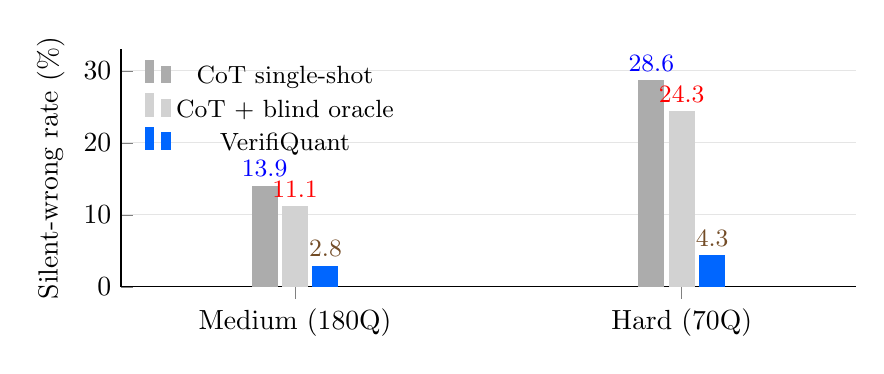
\begin{tikzpicture}
\begin{axis}[
  ybar, bar width=9pt,
  width=0.9\linewidth, height=4.6cm,
  ymin=0, ymax=33,
  ylabel={Silent-wrong rate (\%)},
  ylabel near ticks,
  symbolic x coords={Medium (180Q), Hard (70Q)},
  xtick=data,
  enlarge x limits=0.45,
  legend style={at={(0.02,0.98)}, anchor=north west, font=\small, draw=none, fill=none},
  nodes near coords, nodes near coords style={font=\small},
  tick label style={font=\normalsize},
  label style={font=\normalsize},
  axis lines*=left, ymajorgrids, grid style={gray!20},
]
\addplot+[ybar, fill=gray!65, draw=gray!65] coordinates {(Medium (180Q),13.9) (Hard (70Q),28.6)};
\addplot+[ybar, fill=gray!35, draw=gray!35] coordinates {(Medium (180Q),11.1) (Hard (70Q),24.3)};
\addplot+[ybar, fill=blue!60!cyan, draw=blue!60!cyan] coordinates {(Medium (180Q),2.8) (Hard (70Q),4.3)};
\legend{CoT single-shot, CoT + blind oracle, VerifiQuant}
\end{axis}
\end{tikzpicture}
\caption{Difficulty shift as a governance stress test. Hard-tier questions roughly double CoT's silent-wrong rate under both configurations; VerifiQuant's stays in a narrow band, so its advantage widens from \vqSWRatioMed{} to \vqSWRatioHard{}.}
\label{fig:tiers}
\end{figure}

\section{Design rationale: alternatives we rejected}\label{sec:rationale}
Three designs we prototyped or evaluated en route shaped the final architecture; each fails for a reason that clarifies what the controls actually require.
\emph{(a) One-shot symbolic compilation.}
Compiling all financial logic up front into a solver-executable policy space (SMT-lib policies over accounting and regulatory rules \cite{akinfaderin2025verafi}, or deterministic rule graphs) yields near-perfect logical consistency \emph{after} translation---but a single error in that one-shot translation poisons every downstream execution, and the rigid policy space resists the heterogeneous phrasing of real questions.
FICs amortize formalization per formula family instead: each contract is validated independently at build time, a bad card damages only its own family, and selection keeps a natural-language interface.
\emph{(b) Symbolic-proof transforms.}
Our first transform design attached a computer-algebra proof to each repair (e.g., $\mathrm{PV}_{\mathrm{due}}=\mathrm{PV}_{\mathrm{ord}}\times(1+r)$, checked with a CAS).
We dropped the solver: the proof catalog needs manual maintenance, and the natural-language-to-symbolic translation it depends on is itself the dominant failure mode identified in \S\ref{sec:governance}.
Numerical cross-verification of the declared identity on sampled inputs yields the same accept/reject decision with no symbolic dependency.
\emph{(c) Probabilistic belief fusion.}
Reasoning-in-action systems that anchor claims to calibrated confidence scores answer ``how sure are we?''---but a calibrated 0.85 cannot answer \emph{which check failed}, and finance's near-zero error tolerance demands exact attribution, not belief updates.
The common thread: every rejected design either centralizes a fragile translation step or reports uncertainty without attribution; the funnel decentralizes the former and structurally provides the latter.

\section{Canonical 50Q protocol validation}\label{app:fiftyq}
The 50Q medium subset carries the full baseline grid (Table~\ref{tab:fifty}).
Three findings transfer.
(1)~\emph{Oracle strength does not eliminate silent wrongs}: the strongest leak-free configuration (plain oracle, Pro) reaches 98\% accuracy yet keeps SWR $\geq2\%$; its surviving error is architectural---LLM arithmetic on $2.4^{1/5}$ oscillates across turns (19.11--19.16), which no clarification can fix and deterministic execution computes exactly.
(2)~\emph{A multi-agent system with a human-escalation node never uses it}: the MAS baseline answered all 50 questions without once triggering \texttt{ask\_human} (SWR 14\%)---possessing a checkpoint is not executing one.
Its failure modes, observed during reimplementation, are instructive: after several rounds of inter-agent chatter the base agent starts ignoring provided variables---in one loan case it dropped the stated five-year term entirely; in a Qstick case it \emph{fabricated} input prices from a remembered template instead of parsing the ten values in context---and adding our funnel taxonomy as reflection prompts raised accuracy but induced base--reflection loops rather than escalation to the human node.
(3)~\emph{Iteration is safe under the funnel} (Table~\ref{tab:ablation}): clarification converts abstentions to correct answers but cannot cross a deterministic gate, so oracle budget buys accuracy while the funnel owns safety.
Four independent reruns leave accuracy and SWR identical while the recovery path varies (4--8 oracle triggers)---the precise shape of the C5 guarantee: deterministic layers replay exactly from stored bindings, LLM-mediated paths are logged rather than deterministic, and outcomes are rerun-stable because the funnel, not the path, owns safety.

\begin{table}[t]
\caption{Oracle-budget ablation on the canonical 50Q run (truncation of a single $K{=}3$ run, so rows are self-consistent with the diagnostic distribution). Increasing $K$ only converts abstentions to correct answers; SWR is pinned at 0\% by the deterministic gates.}
\label{tab:ablation}
\small
\begin{tabular}{@{}lrrrr@{}}
\toprule
Budget & Correct & Abstain & SWR & Recovery \\
\midrule
$K{=}1$ (funnel only) & 37 (74\%) & 13 & 0\% & --- \\
$K{=}2$ & 42 (84\%) & 8 & 0\% & $+5$ \\
$K{=}3$ (default) & 45 (90\%) & 5 & 0\% & $+8$ \\
\bottomrule
\end{tabular}
\end{table}
\emph{Card-generation confound, disclosed:} the 50Q pilot used hand-repaired contracts; on the auto-generated cards the same 50 questions scored 49/1/0 before the type audit and 50/0/0 after it, so contract quality---not model choice---is the first-order variable.

\begin{table}[t]
\caption{Canonical 50Q (medium) protocol validation. Blind-review oracles; ternary accounting as \S\ref{sec:protocol} (the single informal no-answer, the same question in three configurations, is footnoted as abstention).}
\label{tab:fifty}
\small
\begin{tabular}{@{}lrrrr@{}}
\toprule
System (Flash unless noted) & Corr. & SW & Abst & SWR \\
\midrule
CoT single-shot & 41 & 8 & 1 & 16.0\% \\
CoT single-shot (Pro) & 41 & 8 & 1 & 16.0\% \\
CoT + plain oracle & 47 & 3 & 0 & 6.0\% \\
CoT + funnel oracle & 46 & 4 & 0 & 8.0\% \\
CoT + plain oracle (Pro) & 49 & 1 & 0 & 2.0\% \\
CoT + funnel oracle (Pro) & 48 & 1 & 1 & 2.0\% \\
JPM MAS reimpl.\ \cite{kundu2025multiagent} & 43 & 7 & 0 & 14.0\% \\
\textbf{VerifiQuant} & \textbf{45} & \textbf{0} & \textbf{5} & \textbf{0.0\%} \\
VerifiQuant (Pro) & 43 & 2 & 5 & 4.0\% \\
\bottomrule
\end{tabular}
\end{table}
